% !TEX encoding = UTF-8
% !TEX TS-program = pdflatex
% !TEX root = ../Tesi.tex

%************************************************

%************************************************


L'argomentazione rappresenta un approccio al ragionamento nei casi in cui si dispone di conoscenza inconsistente, e può essere considerata come un metodo per gestire l’incertezza. Infatti, l’idea alla base dell'argomentazione è quella di valutare il motivo per cui un fatto sia considerato vero analizzando gli argomenti e le relazioni che intercorrono tra essi per valutarne la certezza. Tale processo può essere visto come una forma di ragionamento riguardo gli argomenti per determinarne i più accettabili. Sebbene il termine argomentare possa intuitivamente richiamare diversi significati come quello del ragionamento a partire da premesse fino alle conclusioni o l'esprimere la propria opinione in una discussione, un argomento non si lega a particolari strutture ma in senso astratto è qualsiasi cosa che può attaccare o essere attaccata da un altro argomento. Per tale motivo, un Argumentation Framework può essere adeguato a rappresentare diverse situazioni. La possibilità dell'Argumentation Framework di poter rappresentare diverse situazioni ha portato, nel tempo, alla proposta di estensioni che ponessero attenzione su diversi aspetti, come i tipi di relazione che possono sussistere o la quantificazione della forza di una relazione tra due argomenti.

\section{Argumetation Framework}
La definizione iniziale formulata da Dung prevede esclusivamente la presenza di relazioni di attacco tra argomenti e non permette di assegnare un peso a ciascuna relazione per indicare la forza di un attacco \cite{dung1995acceptability}. Successivamente, tali aspetti sono stati considerati in particolari estensioni dell'AF, come quella del Bipolar Argumentation Framework (BAF), che prevede relazioni di attacco e di supporto tra gli argomenti, e quella del Weighted Argumentation Framework (WAF), in cui le relazioni di attacco sono pesate.


\subsection{Argumetation Framework di Dung}
Si riporta di seguito la descrizione formale dell'argumentation framework di Dung \cite{dung1995acceptability}, che costituisce l’argumentation framework più semplice, contenente solamente relazioni di attacco tra argomenti.

\bigskip
\begin{defn} \textbf{Argumentation Framework (AF)}. Un Argumentation Framework (AF) è una coppia ⟨A,R⟩, dove A è un insieme di argomenti, R ⊆ A × A è una relazione binaria. Dati due argomenti a, b ∈ A, se esiste una coppia ⟨a, b⟩ ∈ R significa che a attacca b. Un insieme S ⊆ A attacca b se b è attaccato da un argomento in S. Un insieme S di argomenti attacca un insieme S' di argomenti se esiste un argomento a ∈ S che attacca un argomento b ∈ S'.
\end{defn}

Un argumentation framework $\mathcal{AF = ⟨A,R⟩}$ può essere rappresentato come un grafo orientato $\mathcal{G = ⟨V, E⟩}$, dove l’insieme dei nodi $\mathcal{V}$ corrisponde all'insieme $\mathcal{A}$ e l’insieme degli archi $\mathcal{E}$ corrisponde all'insieme $\mathcal{R}$.

\bigskip
\begin{exmp}
    Sia dato l'$\mathcal{AF = ⟨A, R⟩}$, dove:
    \begin{center}
        $\mathcal{A} = ⟨a, b, c, d, e, f, g, h⟩$
        
        $\mathcal{R} = \{⟨a, b⟩, ⟨b, c⟩, ⟨c, d⟩, ⟨a, e⟩, ⟨e, d⟩, ⟨e, f ⟩, ⟨f, g⟩, ⟨g, e⟩, ⟨f, h⟩, ⟨h, f ⟩\}$
    \end{center}
    
    \begin{figure}
      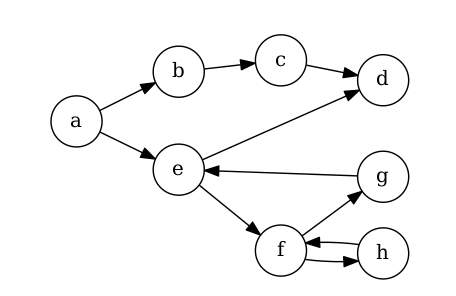
\includegraphics[width=\linewidth]{Immagini/example-graph.png}
      \caption{Rappresentazione del grafo.}
      \label{fig:graph1}
    \end{figure}
    
    \label{exm:af}
\end{exmp}

\bigskip
\begin{defn} \textbf{Difesa} Sia dato un argumentation framework $\mathcal{AF = ⟨A, R⟩}$ Un argomento a $\mathcal{∈ A}$ è difeso da un insieme di argomenti $\mathcal{S ⊆ A} $ e per ogni argomento b  $\mathcal{∈ A}$ vale che se ⟨b, a⟩ $\mathcal{∈ R}$ allora b è attaccato da $\mathcal{S}$.
\end{defn}

Ad esempio, nell'$\mathcal{AF}$ definito nell'esempio \ref{exm:af}, {a} difende c perché b, attaccante di c, è a sua volta attaccato da a.

\bigskip
\begin{defn} \textbf{Conflict-free} Sia dato un argumentation framework AF =
⟨A, R⟩. Un insieme S ⊆ A è conflict-free se e solo se non esistono due argomenti a, b ∈ S tali che ⟨a, b⟩ ∈ R.
\end{defn}  

Ad esempio, nell'$\mathcal{AF}$ definito nell'esempio \ref{exm:af}, \{a, c, g, h\} è conflict-free perché non presenta argomenti in relazione tra di loro.

\bigskip
\begin{defn} \textbf{Stable extension} Sia dato un argumentation framework
$\mathcal{AF = ⟨A, R⟩}$. Un insieme $\mathcal{S ⊆ A}$ conflict-free è una stable extension se e solo se per ogni argomento c $\mathcal{∈ A}$ tale che c $\mathcal{∉ S}$ vale che esiste un argomento b $\mathcal{∈ S}$ tale che ⟨b, c⟩ $\mathcal{∈ R}$.
\end{defn}

Ad esempio, nell'$\mathcal{AF}$ definito nell'esempio \ref{exm:af}, l'insieme delle stable extension è costituito da $\{\{a, c, f \}, \{a, c, g, h\}\}$.

\bigskip
\begin{defn} \textbf{Admissible extension} Sia dato un argumentation framework $\mathcal{AF = ⟨A, R⟩}$. Un insieme $\mathcal{S ⊆ A}$ conflict-free è una admissible extension se e solo se ogni argomento in $\mathcal{S}$ è difeso da $\mathcal{S}$.
\label{adm-ext-dung}
\end{defn}

Ad esempio, nell'$\mathcal{AF}$ definito nell'esempio \ref{exm:af}, l'insieme delle stable extension è costituito da \{∅, \{a\}, \{h\}, \{a, c\}, \{a, f\}, \{a, h\}, \{g, h\}, \{a, c, f \}, \{a, c, h\}, \{a, g, h\},
\{a, c, g, h\}\}.

\bigskip
\begin{defn} \textbf{Preferred extension} Sia dato un argumentation framework $\mathcal{AF = ⟨A, R⟩}$. Un insieme $\mathcal{S ⊆ A}$ è una preferred extension se è una admissible
extension massimale rispetto all'inclusione insiemistica.
\end{defn}

Ad esempio, nell'$\mathcal{AF}$ definito nell'esempio \ref{exm:af}, l'insieme delle preferred extension è costituito da \{\{a, c, f \}, \{a, c, g, h\}\}.

\bigskip
\begin{defn} \textbf{Complete extension} Sia dato un argumentation framework $\mathcal{AF = ⟨A, R⟩}$. Un insieme $\mathcal{S ⊆ A}$ ammissibile è una complete extension se e solo se ogni argomento che è difeso da $\mathcal{S}$ appartiene ad $\mathcal{S}$.
\end{defn}

Ad esempio, nell'$\mathcal{AF}$ definito nell'esempio \ref{exm:af}, l'insieme delle complete extension è costituito da \{\{a, c\}, \{a, c, f \}, \{a, c, g, h\}\}.

\bigskip
\begin{defn} \textbf{Grounded extension} Sia dato un argumentation framework $\mathcal{AF = ⟨A, R⟩}$. Un insieme $\mathcal{S ⊆ A}$ è la grounded extension se è una complete extension minimale rispetto all'inclusione insiemistica.
\end{defn}

Ad esempio, nell'$\mathcal{AF}$ definito nell'esempio \ref{exm:af}, la grounded extension è costituita da \{\{a, c\}\}.

\bigskip
\begin{prp}Ogni stable extension è anche una preferred extension, ma non il contrario. Inoltre, ogni preferred extension è anche una complete extension. Possono esistere più stable, preferred e complete extension, ma la grounded extension è unica.
\end{prp}

Per quanto riguarda i cicli presenti in un argumentation framework, valgono le seguenti proprietà:

\bigskip
\begin{prp}. Se un argumentation framework $\mathcal{AF = ⟨A,R⟩}$ non ha alcun ciclo di lunghezza pari, allora l’unica preferred extension di AF è l’insieme vuoto.
\end{prp}

\bigskip
\begin{prp}. Se un argumentation framework $\mathcal{AF = ⟨A,R⟩}$ non ha alcun ciclo di lunghezza dispari, allora ogni preferred extension di AF è una stable extension.
\end{prp}

\bigskip
\begin{prp}. Se un argumentation framework $\mathcal{AF = ⟨A,R⟩}$ non ha alcun ciclo ed $\mathcal{A = ∅}$, allora $\mathcal{AF}$ ha una singola estensione che è preferred, completa e grounded.
\end{prp}


\subsection{Bipolar Argumetation Framework}
Una estensione dell'argumentation framework di Dung considera il fatto che tra due argomenti non esiste solo una relazione di attacco, ma può esistere anche una relazione di supporto. La distinzione in due tipi di relazioni opposte tra di loro suggerisce la nozione di bipolarismo, ovvero l’esistenza di due tipi di informazioni indipendenti che hanno natura diametralmente opposta e che rappresentano forze di repulsione. Il concetto di bipolarismo è importante quando si devono prendere decisioni in quanto è possibile distinguere informazioni a supporto di una decisione, ed informazioni che la contrastano [1]. Si descrive, di seguito, formalmente il bipolar argumentation framework.

\bigskip
\begin{defn} \textbf{Bipolar Argumentation Framework (BAF)} Un Bipolar Argumentation Framework (BAF) è una tripla $⟨\mathcal{A}, \mathcal{R}_{def}, \mathcal{R}_{sup}⟩$ dove $\mathcal{A}$ è un insieme di argomenti, $\mathcal{R}_{def}$ è una relazione binaria su $\mathcal{A}$ chiamata relazione di attacco e $\mathcal{R}_{sup}$ è una relazione binaria su $\mathcal{A}$ chiamata relazione di supporto. Dati due argomenti $a, b ∈ \mathcal{A}$, $a \mathcal{R}_{def} b ⇔ ⟨a, b⟩ ∈ \mathcal{R}_{def}$ (rispettivamente  $a \mathcal{R}_{sup} b ⇔ ⟨a, b⟩ ∈  \mathcal{R}_{sup}$ ) indica che a attacca b (rispettivamente a supporta b). Un bipolar argumentation framework $BAF = ⟨\mathcal{A}, \mathcal{R}_{def} , \mathcal{R}_{sup} ⟩$ può essere rappresentato come un grafo orientato $\mathcal{G} = ⟨\mathcal{V}, \mathcal{E}⟩$, dove l'insieme dei nodi $\mathcal{V}$ corrisponde all'insieme $\mathcal{A}$ e l'insieme degli archi $\mathcal{E}$ corrisponde all'insieme $\mathcal{R}_{def} ∪ \mathcal{R}_{sup}$. Dati due argomenti $a, b ∈ \mathcal{A}$, $a \mathcal{R}_{def} b$ è rappresentato come $a → b$ e $a \mathcal{R}_{sup} b$ è rappresentato come $a -→ b$.

\end{defn}

\bigskip
\begin{exmp}
    Sia dato il $BAF  = ⟨\mathcal{A}, \mathcal{R}_{def}, \mathcal{R}_{sup}⟩$, dove:
    \begin{center}
        $\mathcal{A} = ⟨a, b, c, d, e, f, g, h⟩$
        
        $\mathcal{R}_{def} = \{⟨c, d⟩, ⟨a, e⟩, ⟨e, f⟩, ⟨f, g⟩, ⟨g, e⟩, ⟨f, h⟩, ⟨h, f⟩\}$
        
        $\mathcal{R}_{sup} = \{⟨a, b⟩, ⟨b, c⟩, ⟨e, d⟩\}$
    \end{center}
    
    \begin{figure}
      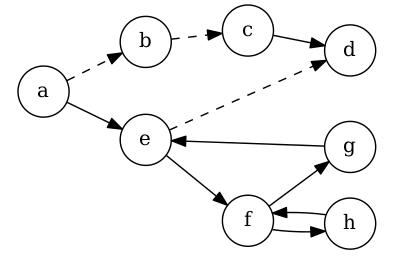
\includegraphics[width=\linewidth]{Immagini/example-baf-graph.png}
      \caption{Rappresentazione del grafo bipolar.}
      \label{fig:baf-graph1}
    \end{figure}
    
    \label{exm:baf}
\end{exmp}

\bigskip
\begin{defn} \textbf{Relazione di Attacco Diretto} 
Sia dato un bipolar argumentation framework $BAF = ⟨\mathcal{A}, \mathcal{R}_{def}, \mathcal{R}_{sup}⟩$ e siano dati due argomenti $a, b ∈ \mathcal{A}$. Se $ a \mathcal{R}_{def} b$ allora si parla di attacco diretto da a verso b.
\end{defn}

Ad esempio, nel $BAF$ definito nell'esempio \ref{exm:baf}, è presente una relazione di attacco diretto da $c$ verso $d$ perchè $⟨c, d⟩ ∈ \mathcal{R}_{def}$.


\bigskip
\begin{defn} \textbf{Relazione di Attacco Indiretto} 
Sia dato un bipolar argumentation framework $BAF = ⟨\mathcal{A}, \mathcal{R}_{def}, \mathcal{R}_{sup}⟩$. Un attacco indiretto verso un argomento $b ∈ \mathcal{A}$ è una sequenza $a_{1}\mathcal{R}_{1}...\mathcal{R}_{n-1}a_{n}$ dove $n \geq 3, a_n = b, \forall i = 2, ..., n-1, \mathcal{R}_i = \mathcal{R}_{sup}$ e $ \mathcal{R}_{1} = \mathcal{R}_{def}$.
\end{defn}

Ad esempio, nel $BAF$ definito nell'esempio \ref{exm:baf}, è presente una relazione di attacco indiretto verso $d$ perchè $⟨a, e⟩ ∈ \mathcal{R}_{def}$ e $⟨e, d⟩ ∈ \mathcal{R}_{sup}$.


\bigskip
\begin{defn} \textbf{Attacco supportato} 
Sia dato un bipolar argumentation framework $BAF = ⟨\mathcal{A}, \mathcal{R}_{def}, \mathcal{R}_{sup}⟩$. Un attacco supportato verso un argomento $b ∈ \mathcal{A}$ è una sequenza $a_{1}\mathcal{R}_{1}...\mathcal{R}_{n-1}a_{n}$ dove $n \geq 3, a_n = b, \forall i = 1, ..., n-2, \mathcal{R}_i = \mathcal{R}_{sup}$ e $ \mathcal{R}_{n-1} = \mathcal{R}_{def}$.
\end{defn}

Ad esempio, nel $BAF$ definito nell'esempio \ref{exm:baf}, è presente un attacco supportato verso $d$ perchè $⟨c, d⟩ ∈ \mathcal{R}_{def}$ e $⟨a, b⟩, ⟨b, c⟩ ∈ \mathcal{R}_{sup}$.


\bigskip
\begin{defn} \textbf{Attacco di insieme} 
Sia dato un bipolar argumentation framework $BAF = ⟨\mathcal{A}, \mathcal{R}_{def}, \mathcal{R}_{sup}⟩$. Un insieme $S \subseteq A$ attacca un argomento $b \in A$ se e solo se esiste un attacco diretto, supportato o indiretto verso $b$ da un elemento di $S$.
\end{defn}

Ad esempio, nel $BAF$ definito nell'esempio \ref{exm:baf}, è presente un attacco di insieme da $S = =\{a, b, c\}$ verso $d$ perchè esiste un attacco supportato dagli elementi $a, b, c \in S$ verso $d$.


\bigskip
\begin{defn} \textbf{Supporto di insieme} 
Sia dato un bipolar argumentation framework $BAF = ⟨\mathcal{A}, \mathcal{R}_{def}, \mathcal{R}_{sup}⟩$. Un insieme $S \subseteq A$ supporta un argomento $b \in A$ se e solo se esiste una sequenza $a_{1}\mathcal{R}_{sup}...\mathcal{R}_{sup}a_{n}$ dove $n \geq 2, a_n = b$ e $a_1 \in S$
\end{defn}

Ad esempio, nel $BAF$ definito nell'esempio \ref{exm:baf}, è presente un supporto di insieme da $S = =\{a\}$ verso $c$ perchè esiste una sequenza di supporti da $a \in S$ verso $c$.


\bigskip
\begin{defn} \textbf{Difesa} 
Sia dato un bipolar argumentation framework $BAF = ⟨\mathcal{A}, \mathcal{R}_{def}, \mathcal{R}_{sup}⟩$. Un insieme $S \subseteq A$ difende un argomento $a \in A$ se e solo se per ogni argomento $b \in A$, se $b$ attacca $a$ allora $b$ è attaccato da $S$.
\end{defn}

Ad esempio, nel $BAF$ definito nell'esempio \ref{exm:baf}, $e$ difende $g$ perchè $f$, attaccante di $g$, è a sua volta attaccato da $e$.


\bigskip
\begin{defn} \textbf{Conflict-free} 
Sia dato un bipolar argumentation framework $BAF = ⟨\mathcal{A}, \mathcal{R}_{def}, \mathcal{R}_{sup}⟩$. Un insieme $S \subseteq A$ è conflict-free se e solo se non esistono due argomenti $a, b \in S$ tali che sussista un attacco di insieme da $\{a\}$ verso $b$.
\end{defn}

Ad esempio, nel $BAF$ definito nell'esempio \ref{exm:baf}, $\{a, b, c, f\}$ è conflict-free perchè non presenta argomenti coinvolti in attacchi di insieme tra loro.


\bigskip
\begin{defn} \textbf{Safe} 
Sia dato un bipolar argumentation framework $BAF = ⟨\mathcal{A}, \mathcal{R}_{def}, \mathcal{R}_{sup}⟩$. Un insieme $S \subseteq A$ è safe se e solo se non esiste alcun argomento $b \in A$ tale che sussista un attacco di insieme da $\{S\}$ verso $b$ o che ci sia un supporto di insieme da $S$ verso $b$ o che $b \in S$. 
\end{defn}

Ad esempio, nel $BAF$ definito nell'esempio \ref{exm:baf}, $\{b, c\}$ è safe perchè attacca solo $d$, ma non lo supporta; inoltre $d$ non appartiene a tale insieme.


\bigskip
\begin{defn} \textbf{Stable Extension} 
Sia dato un bipolar argumentation framework $BAF = ⟨\mathcal{A}, \mathcal{R}_{def}, \mathcal{R}_{sup}⟩$. Un insieme $S \subseteq A$ conflict-free è una stable extension se e solo se per ogni argomento $a \notin S$ sussiste un attacco di insieme da $S$ verso $a$.
\end{defn}

Ad esempio, nel $BAF$ definito nell'esempio \ref{exm:baf}, l'insieme delle stable extension è costituito da $\{\{a, b, c, f\}, \{a, b, c, g, h\}\}$.


\bigskip
\begin{defn} \textbf{d-admissible extension} 
Sia dato un bipolar argumentation framework $BAF = ⟨\mathcal{A}, \mathcal{R}_{def}, \mathcal{R}_{sup}⟩$. Un insieme $S \subseteq A$ conflict-free è una d-admissible extension se e solo se ogni argomento in $S$ è difeso da $S$. Tale definizione equivale alla definizione \ref{adm-ext-dung} di ammissibilità per l'AF di Dung.
\end{defn}

Ad esempio, nel $BAF$ definito nell'esempio \ref{exm:baf}, l'insieme delle d-admissible extension è costituito da $\{∅, \{a, h\}$, $\{a, b, h\}$, $\{a, c, h\}$, $\{a, b, c, h\}$, $\{a, g, h\}$, $\{a, b, g, h\}$, $\{a, c, g, h\}$, $\{a, b, c, g, h\}$, $\{g, h\}$, $\{c, g, h\}$, $\{b, g, h\}$, $\{b, c, g, h\}$, $\{b, h\}$, $\{b, c, h\}$, $\{c, h\}$, $\{h\}$, $\{a, f\}$, $\{a, b, f \}$, $\{a, c, f \}$, $\{a, b, c, f \}$, $\{a\}$, $\{a, b\}$, $\{a, c\}$, $\{a, b, c\}$, $\{b\}$, $\{b, c\}$, $\{c\}\}$.


\bigskip
\begin{defn} \textbf{s-admissible extension} 
Sia dato un bipolar argumentation framework $BAF = ⟨\mathcal{A}, \mathcal{R}_{def}, \mathcal{R}_{sup}⟩$. Un insieme $S \subseteq A$ safe è una s-admissible extension se e solo se ogni argomento in $S$ è difeso da $S$.
\end{defn}

Ad esempio, nel $BAF$ definito nell'esempio \ref{exm:baf}, l'insieme delle s-admissible extension è costituito da $\{∅, \{a, h\}$, $\{a, b, h\}$, $\{a, c, h\}$, $\{a, b, c, h\}$, $\{a, g, h\}$, $\{a, b, g, h\}$, $\{a, c, g, h\}$, $\{a, b, c, g, h\}$, $\{g, h\}$, $\{c, g, h\}$, $\{b, g, h\}$, $\{b, c, g, h\}$, $\{b, h\}$, $\{b, c, h\}$, $\{c, h\}$, $\{h\}$, $\{a, f \}$, $\{a, b, f \}$, $\{a, c, f \}$, $\{a, b, c, f \}$, $\{a\}$, $\{a, b\}$, $\{a, c\}$, $\{a, b, c\}$, $\{b\}$, $\{b, c\}$, $\{c\}\}$.


\bigskip
\begin{defn} \textbf{c-admissible extension}
Sia dato un bipolar argumentation framework $BAF = ⟨\mathcal{A}, \mathcal{R}_{def}, \mathcal{R}_{sup}⟩$. Un insieme $S \subseteq A$ conflict-free è una c-admissible extension se e solo se $S$ è chiuso rispetto ad $\mathcal{R}_{sup}$ ed ogni argomento in $S$ è difeso da $S$.
\end{defn}

Ad esempio, nel $BAF$ definito nell'esempio \ref{exm:baf}, l'insieme delle c-admissible extension è costituito da $\{∅, \{a, b, c, f \}$, $\{a, b, c, h\}$, $\{a, b, c, g, h\}$, $\{a, b, c\}$, $\{g, h\}$, $\{h\}\}$.


\bigskip
\begin{defn} \textbf{d-preferred (risp. s-preferred, c-preferred) extension}
Sia dato un bipolar argumentation framework $BAF = ⟨\mathcal{A}, \mathcal{R}_{def}, \mathcal{R}_{sup}⟩$. Un insieme $S \subseteq A$ è una d-preferred (risp. s-preferred, c-preferred) extension se è una d-admissible (risp. s-admissible, c-admissible) extension massimale rispetto all'inclusione insiemistica.
\end{defn}

Ad esempio, nel $BAF$ definito nell'esempio \ref{exm:baf}, l'insieme delle d-preferred, s-preferred, c-preferred extension sono tutti costituiti da $\{\{a,b,c,g,h\}$, \\ $\{a,b,c,f\}\}$.



\begin{table}[H]
    \centering
    \begin{tabular}{|l|c|c|}
        \hline
        \textbf{Extension} & \textbf{\textit{AF}} & \textit{\textbf{BAF}} \\ \hline
        \textbf{Stable}       & x & x \\ \hline
        \textbf{d-admissible} & x & x \\ \hline
        \textbf{s-admissible} &   & x \\ \hline
        \textbf{c-admissible} &   & x \\ \hline
        \textbf{Complete}     & x &   \\ \hline
        \textbf{Grounded}     & x &   \\ \hline
        \textbf{d-preferred}  & x & x \\ \hline
        \textbf{s-preferred}  &   & x \\ \hline
        \textbf{c-preferred}  &   & x \\ \hline
    \end{tabular}
    \caption{Tabella di riepilogo delle estensioni calcolabili per \textit{AF} e \textit{BAF}.}
\end{table}


\subsection{Weighted Argumetation Framework}
Una ulteriore proposta che segue una direzione differente è l'estensione dell'argumentation framework di Dung in cui gli attacchi tra argomenti sono associati ad un peso numerico che indica la forza di un attacco. Ad esempio, si considerino i seguenti argomenti:

\begin{itemize}
    \item \textbf{a1} "The house is in a good location, it is large enough for our family and it is affordable: we should buy it".
    \item \textbf{a2} "The house suffers from subsidence, which would be prohibitively expensive to fix: we should not buy it".
\end{itemize}

Entrambi gli argomenti si attaccano a vicenda poiché in contrasto tra di loro, per cui nel caso dell'argumentation framework di Dung non sarà possibile individuare una estensione grounded. Infatti, tale rappresentazione non tiene conto del fatto che gli attacchi non hanno uguale peso. Nell'esempio riportato, \textbf{a2} attacca in modo più forte \textbf{a1}, per cui tale attacco assume un peso maggiore. Considerando tali pesi, viene introdotto un parametro $\beta$, denominato inconsistency budget, con l'obiettivo di filtrare le relazioni ed ottenere una soluzione diversa, in cui determinati argomenti possono essere considerati accettabili rispetto ad una soglia di tolleranza dell'inconsistenza \cite{dunne2011weighted}. Di seguito si descrivono formalmente il Weighted Argumentation Framework e l'inconsistency budget.


\begin{defn} \textbf{Weighted Argumentation Framework (WAF)}
Un Weighted Argumentation Framework $(WAF)$ è una tripla $⟨\mathcal{A}, \mathcal{R}, w⟩$, dove $⟨\mathcal{A}, \mathcal{R}⟩$ è un Argumentation Framework di Dung e $w: \mathcal{R} \rightarrow \mathbb{R}^{+}$ è una funzione che assegna numeri reali strettamente positivi come peso agli attacchi.
\end{defn}

Un Weighted Argumentation Framework $WAF = ⟨\mathcal{A}, \mathcal{R}, w⟩$ può essere rappresentato come un grafo orientato e pesato $\mathcal{G} = ⟨\mathcal{V}, \mathcal{E}⟩$, dove l'insieme dei nodi $\mathcal{V}$ corrisponde all'insieme $\mathcal{A}$ e l'insieme degli archi $\mathcal{E}$ corrisponde all'insieme $\mathcal{R}$.

\begin{exmp}
    Sia dato il $WAF  = ⟨\mathcal{A}, \mathcal{R}, w⟩$, dove:
    \begin{center}
        $\mathcal{A} = ⟨a, b, c, d, e, f, g, h⟩$
        
        $\mathcal{R} = \{⟨a, b⟩, ⟨b, c⟩, ⟨c, d⟩, ⟨a, e⟩, ⟨e, d⟩, ⟨e, f⟩, ⟨f, g⟩, ⟨g, e⟩, ⟨f, h⟩, ⟨h, f⟩\}$
        
        $w(⟨a, b⟩) = 2, w(⟨b, c⟩) = 1, w(⟨c, d⟩) = 3, w(⟨a, e⟩) = 5, w(⟨e, d⟩) = 7, w(⟨e, f⟩) = 2, w(⟨f, g⟩) = 2, w(⟨g, e⟩) = 3, w(⟨f, h⟩) = 5, w(⟨h, f⟩) = 7$
    \end{center}
    
    \begin{figure}[h]
      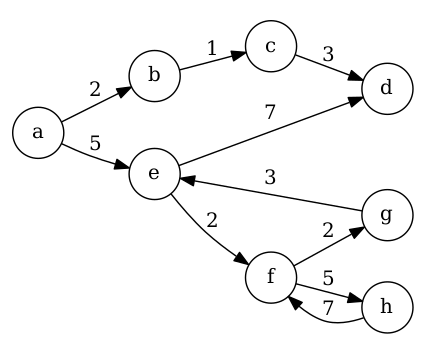
\includegraphics[width=\linewidth]{Immagini/example-waf-graph.png}
      \caption{Rappresentazione del grafo weighted.}
      \label{fig:baf-graph1}
    \end{figure}
    
    \label{exm:waf}
\end{exmp}

Ad esempi nel $WAF$ definito nel'esempio \ref{exm:waf}, linsieme delle admissible extension è costituito da \{∅, \{a, c, f \}$, $\{a, f \}$, $\{a, c\}$, $\{a\}$, $\{g, h\}$, $\{h\}$, $\{a, c, g, h\}$, $\{a, c, h\}$, $\{a, g, h\}$, $\{a, h\}\}. L'insieme delle preferred extension è costituito da $\{\{a, c, f\}$, $\{a, c, g, h\}\}$. L'insieme delle complete extension è costituito da $\{\{a, c, g, h\}$, $\{a, c\}, \{a, c, f\}\}$. La grounded extension è costituita da $\{\{a, c\}\}$.


\section{Argumetation Mining}
L'Argumentation Mining fornisce metodi per l'estrazione di argomenti da documenti testuali ed include molteplici sotto task come la identificazione degli argomenti e la scoperta della loro struttura. Molti ricercatori hanno già applicato l'Argumentation Mining in molti domini. Ad esempio in \cite{teufel1999annotation} si cerca di identificare argomenti nelle frasi di pubblicazioni scientifiche, in \cite{moens2007automatic} gli argomenti vengono estratti da documenti legali, in \cite{feng2011classifying} vengono analizzati articoli di giornale o in \cite{florou2013argument} nelle trascrizioni di casi giudiziari.
